%versi 3 (22-07-2020)
\chapter{Landasan Teori}
\label{chap:teori}
Pada bab ini akan menjelaskan dasar teori mengenai Portal Akademik Mahasiswa dan Selenium. 

\section{Portal Akademik Mahasiswa 2018}
\label{sec:pam} 
Portal Akademik Mahasiswa (selanjutnya disingkat dengan PAM) adalah sebuah \textit{web} yang di peruntukan bagi mahasiswa dalam rangka mendapatkan informasi kegiatan akademik mulai dari registrasi, melihat jadwal kuliah dan ujian, info nilai sampai pendaftaran sidang\cite{portalunpar}. Portal Akademik Mahasiswa dapat diakses melalui \url{https://www.studentportal.unpar.ac.id/}. Pada masa pandemi Covid-19 ini Portal Akademik Mahasiswa UNPAR sudah dapat melakukan perekaman kehadiran secara online melalui \textit{web} Portal Akademik Mahasiswa. Mahasiswa harus \textit{login} dengan \textit{email} dan \textit{passowrd} agar bisa melakukan perekaman kehadiran online.

Panduan untuk melakukan perekaman kehadiran online di Portal Akademik Mahasiswa 2018 sebagai berikut:
\begin{enumerate}
	\item Masuk ke \textit{web} \url{https://www.studentportal.unpar.ac.id/} (Gambar \ref{fig:studpor_home}). Lalu klik tombol \textit{Login}.
		\begin{figure}[H]
		\centering
		
\includegraphics[scale=0.3]{Gambar/halamanWeb.jpg}
		\caption{Tampilan halaman awal Portal Akademik Mahasiswa} 
		\label{fig:studpor_home}
	\end{figure}
	
	\vspace{2cm}
	\item \textit{Login} dengan memasukan \textit{email} mahasiswa unpar dan \textit{password} \ref{fig:pam_login}).
	\begin{figure}[H]
		\centering
		
\includegraphics[scale=0.3]{Gambar/login.jpg}
		\caption{Tampilan halaman untuk melakukan \textit{Login}} 
		\label{fig:pam_login}
	\end{figure}
	
	\item Setelah \textit{login} berhasil dilakukan, maka akan muncul halaman utama (Gambar \ref{fig:pam_home}). Lalu klik pada heksagon berlabel `Jadwal \& Kehadiran' untuk melakukan perekaman kehadiran online.
	\begin{figure}[H]
		\centering
		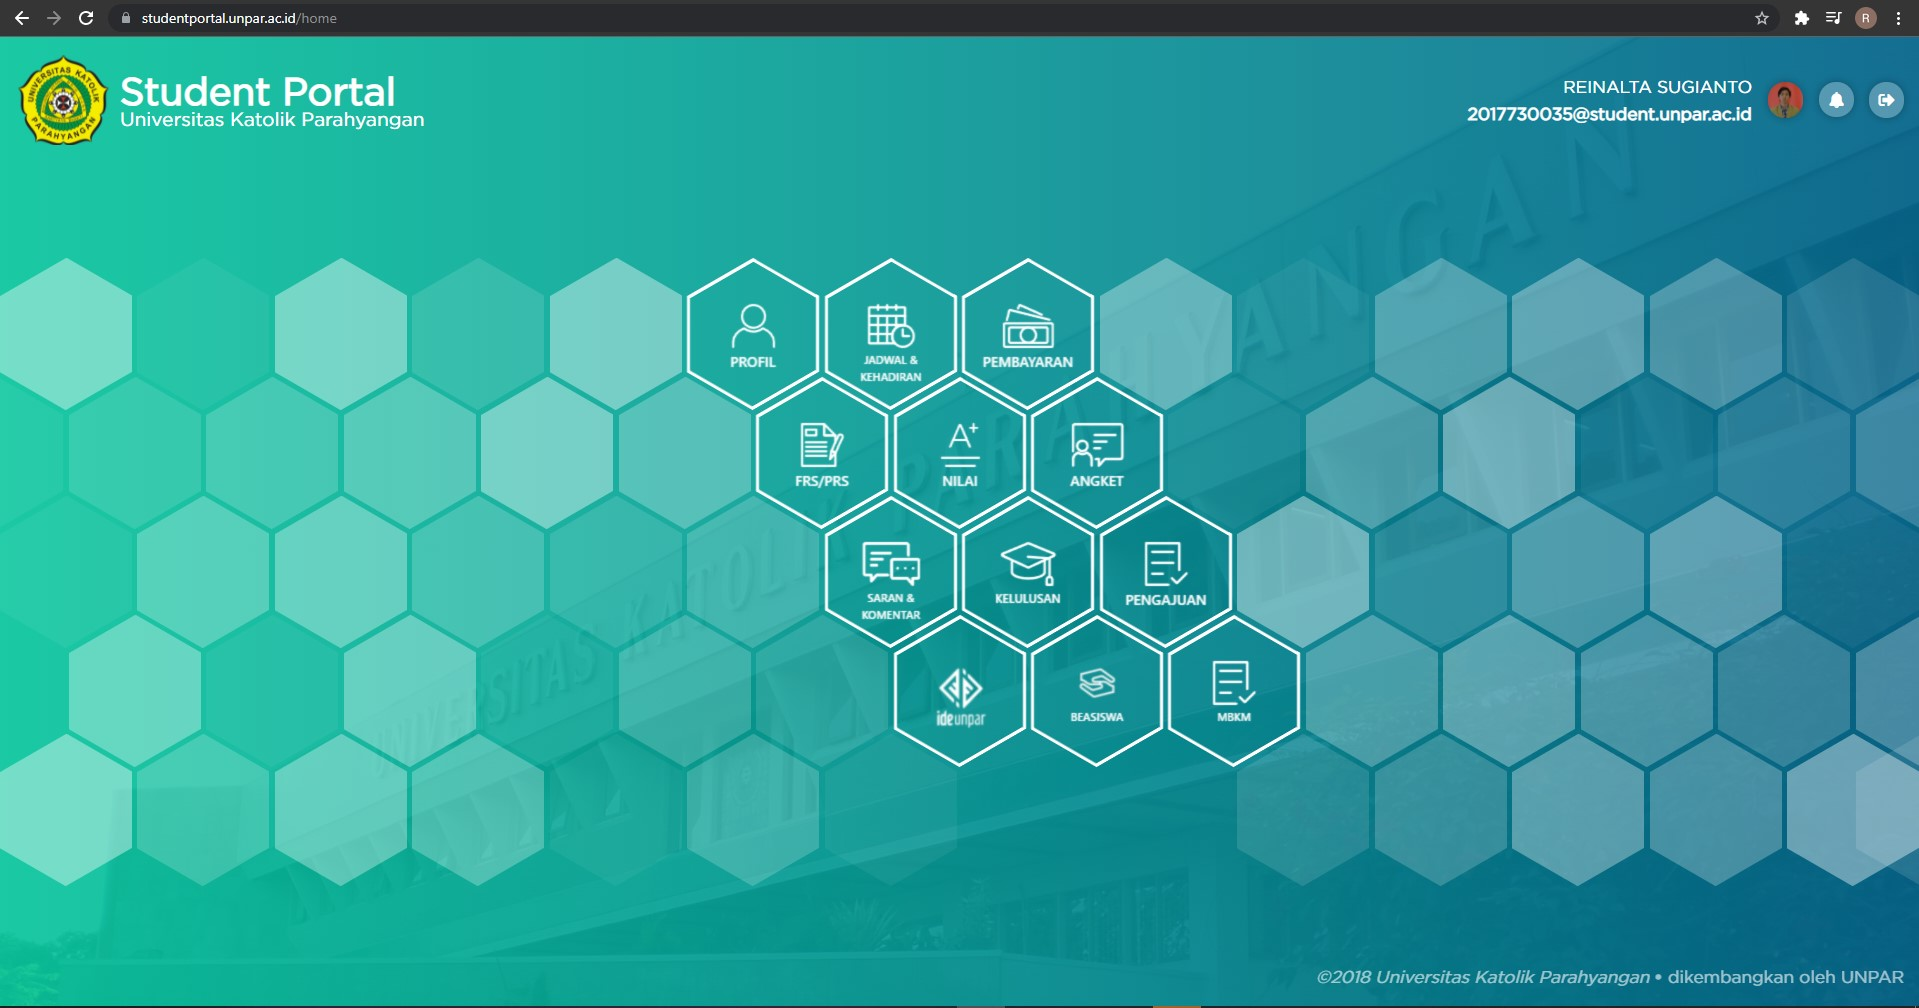
\includegraphics[scale=0.3]{Gambar/jadwalkehadiran.jpg}
		\caption{Tampilan halaman utama Portal Akademik Mahasiswa} 
		\label{fig:pam_home}
	\end{figure}

	\vspace{5cm}
	\item Browser akan menampilkan halaman utama pada fitur `Jadwal \& Kehadiran' (Gambar \ref{fig:pam_kehadiran}). Mahasiswa dapat melihat jadwal kuliah untuk besok hari. Lalu terdapat tombol merah pada kolom presensi untuk melakukan perekaman kehadiran.
	\begin{figure}[H]
		\centering
		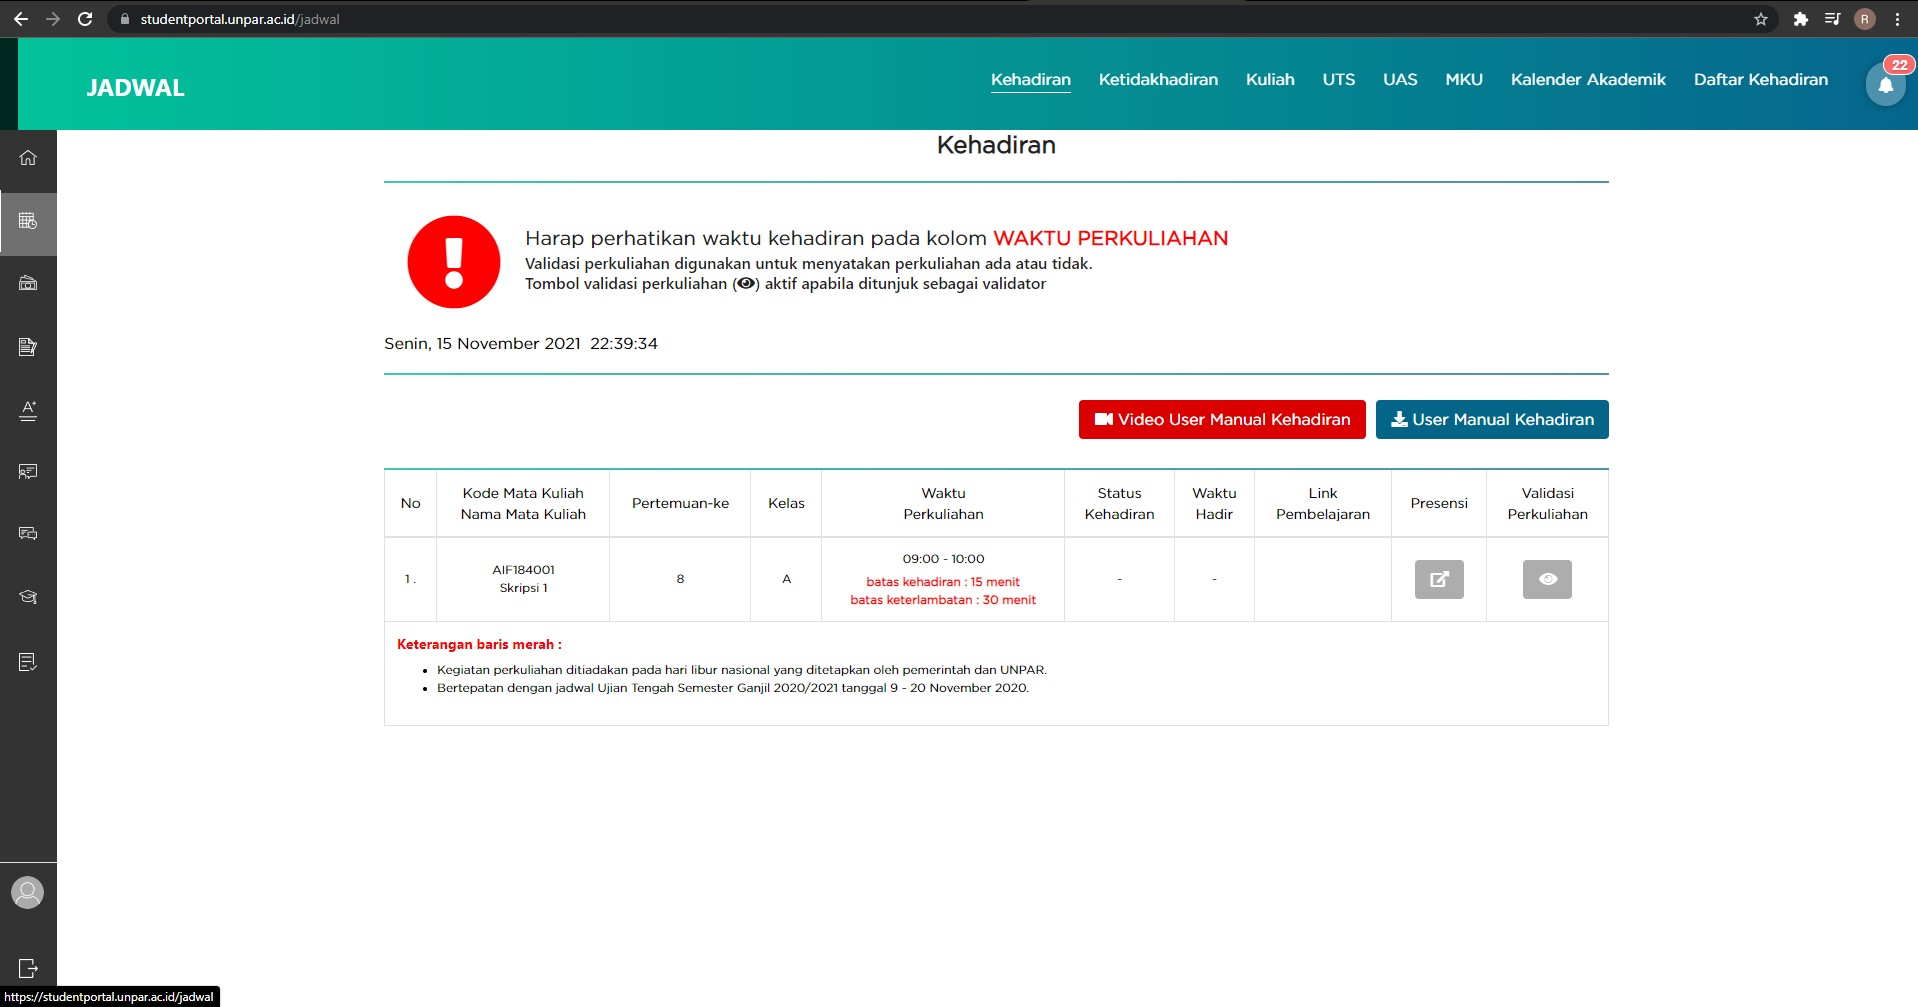
\includegraphics[scale=0.3]{Gambar/kehadiran.jpg}
		\caption{Tampilan halaman untuk melakukan perekam kehadiran online} 
		\label{fig:pam_kehadiran}
	\end{figure}
\end{enumerate}

\section{Selenium}
\label{sec:selenium}
Selenium adalah \textit{open-source} \textit{framework} pengujian otomatisasi untuk aplikasi web\cite{selenium}. WebDriver menggunakan API otomatisasi \textit{browser} yang disediakan oleh vendor \textit{browser} untuk mengontrol \textit{browser} dan melakukan pengujian. API WebDriver ini seolah-olah membuat pengguna secara langsung mengoperasi \textit{browser}, padahal dijalankan secara otomatis langsung oleh \textit{API} WebDriver tersebut. Selenium WebDriver adalah sebuah \textit{tools} yang berguna untuk melakukan otomatisasi terhadap web pada \textit{browser}. Selenium WebDriver ini tersedia untuk bahasa pemrograman Ruby, Java, Python, C\#, dan JavaScript.

\subsection{Navigating}
Hal pertama untuk menggunakan WebDriver adalah menavigasi ke \textit{link}. Cara normal untuk melakukan navigasi adalah dengan \textit{method} \textit{get}().

\subsection{Locating Elements}
Pada selenium ada berbagai cara untuk menemukan elemen di halaman. Selenium menyediakan berbagai metode menemukan elemen yang dapat pilih untuk menyelesaikan kasus tertentu, berikut berbagai metode untuk menemukan elemen:
\begin{enumerate}
	\item find\_element\_by\_id: untuk mencari elemen berdasarkan \textit{id} atribut.
	\item find\_element\_by\_name: untuk mencari elemen berdasarkan nama atribut.
	\item find\_element\_by\_xpath: untuk mencari elemen berdasarkan \textit{xpath}. \textit{XPath} adalah bahasa yang digunakan untuk menemukan node dalam dokumen XML.
	\item find\_element\_by\_link\_text: digunakan untuk mengetahui \textit{link} teks yang digunakan dalam \textit{anchor} tag. Cara ini, elemen pertama dengan \textit{link} teks lengkap yang cocok dengan nilai yang diberikan akan dikembalikan. 
	\item find\_element\_by\_partial\_link\_text: digunakan untuk mengetahui \textit{link} teks yang digunakan dalam \textit{anchor} tag. Cara ini, elemen pertama dengan \textit{link} teks sebagian yang cocok dengan nilai yang diberikan akan dikembalikan. 
	\item find\_element\_by\_tag\_name: untuk mencari elemen berdasarkan nama tag.
	\item find\_element\_by\_class\_name: untuk mencari elemen berdasarkan nama kelas
	\item find\_element\_by\_css\_selector: untuk mencari elemen dengan menggunakan sintaks \textit{CSS selector}
\end{enumerate}
Untuk menemukan beberapa elemen secara langsung, dengan cara berikut:
\begin{enumerate}
	\item find\_elements\_by\_id
	\item find\_elements\_by\_name
	\item find\_elements\_by\_xpat
	\item find\_elements\_by\_link\_text
	\item find\_elements\_by\_partial\_link\_text
	\item find\_elements\_by\_tag\_name
	\item find\_elements\_by\_class\_name
	\item find\_elements\_by\_css\_selector
\end{enumerate}

\subsection{Waits}
Selenium WebDriver menyediakan dua jenis \textit{waits} adalah implisit dan eksplisit. \textit{Waits} eksplisit ini membuat WebDriver menunggu kondisi tertentu terjadi sebelum melanjutkan eksekusi. \textit{Waits} implisit membuat WebDriver melakukan polling DOM untuk jangka waktu tertentu saat mencoba menemukan elemen.

\subsection{WebDriver API}
WebDriver API ini mencakup semua \textit{interface} Selenium WebDriver. Selenium WebDriver dapat digunakan dengan melakukan import webdriver. API pada selenium ini untuk menunjukan lokasi kelas yang absolut, misalkan untuk Firefox, Chrome, Opera, Ie, dan lain-lainnya.

\section{Sistem Perekam Kehadiran}
\label{sec:sistem}





